\documentclass{standalone}
\usepackage{tikz}

\begin{document}
 	\begin{tikzpicture}
 		\draw (5, 5) node[opacity=0.7] {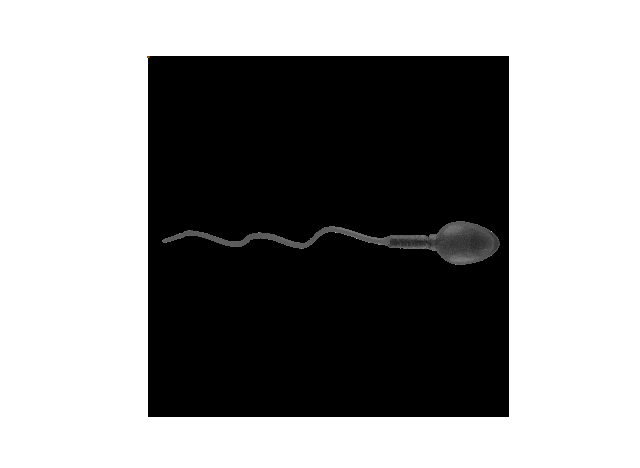
\includegraphics{images/original_gs.png}};
 		%\draw[fill=black](0,0)--(5,0)--(5,5)--(5,0)--(0,0);
 		%\draw[ fill=black!20!white]  (0,0) grid (5,5) rectangle (0,0);
 		\draw[white] (0,0) grid (10,10) ;
 		\draw[gray, name=above] (10,0) -- (0,10);
  		\draw[gray, name=below] (9.5,-0.5) -- (-0.5,9.5);
  		\draw[gray, fill=gray, opacity=0.5] (4,5) -- (5,4) -- (5,5) -- (5,5);
  		\draw[gray] (10,0)--(10.2,0.2)--(10.2,-0.7)--(9.3,-0.7)-- (9.5,-0.5);
  		\draw[gray] (-0.5,9.5)-- (0,10);
  		\node[white,below left] at (5,5) {$a_{ij}$};
   		
 	\end{tikzpicture}
\end{document}
